\documentclass[twoside]{book}

% Packages required by doxygen
\usepackage{fixltx2e}
\usepackage{calc}
\usepackage{doxygen}
\usepackage[export]{adjustbox} % also loads graphicx
\usepackage{graphicx}
\usepackage[utf8]{inputenc}
\usepackage{makeidx}
\usepackage{multicol}
\usepackage{multirow}
\PassOptionsToPackage{warn}{textcomp}
\usepackage{textcomp}
\usepackage[nointegrals]{wasysym}
\usepackage[table]{xcolor}

% Font selection
\usepackage[T1]{fontenc}
\usepackage[scaled=.90]{helvet}
\usepackage{courier}
\usepackage{amssymb}
\usepackage{sectsty}
\renewcommand{\familydefault}{\sfdefault}
\allsectionsfont{%
  \fontseries{bc}\selectfont%
  \color{darkgray}%
}
\renewcommand{\DoxyLabelFont}{%
  \fontseries{bc}\selectfont%
  \color{darkgray}%
}
\newcommand{\+}{\discretionary{\mbox{\scriptsize$\hookleftarrow$}}{}{}}

% Page & text layout
\usepackage{geometry}
\geometry{%
  a4paper,%
  top=2.5cm,%
  bottom=2.5cm,%
  left=2.5cm,%
  right=2.5cm%
}
\tolerance=750
\hfuzz=15pt
\hbadness=750
\setlength{\emergencystretch}{15pt}
\setlength{\parindent}{0cm}
\setlength{\parskip}{3ex plus 2ex minus 2ex}
\makeatletter
\renewcommand{\paragraph}{%
  \@startsection{paragraph}{4}{0ex}{-1.0ex}{1.0ex}{%
    \normalfont\normalsize\bfseries\SS@parafont%
  }%
}
\renewcommand{\subparagraph}{%
  \@startsection{subparagraph}{5}{0ex}{-1.0ex}{1.0ex}{%
    \normalfont\normalsize\bfseries\SS@subparafont%
  }%
}
\makeatother

% Headers & footers
\usepackage{fancyhdr}
\pagestyle{fancyplain}
\fancyhead[LE]{\fancyplain{}{\bfseries\thepage}}
\fancyhead[CE]{\fancyplain{}{}}
\fancyhead[RE]{\fancyplain{}{\bfseries\leftmark}}
\fancyhead[LO]{\fancyplain{}{\bfseries\rightmark}}
\fancyhead[CO]{\fancyplain{}{}}
\fancyhead[RO]{\fancyplain{}{\bfseries\thepage}}
\fancyfoot[LE]{\fancyplain{}{}}
\fancyfoot[CE]{\fancyplain{}{}}
\fancyfoot[RE]{\fancyplain{}{\bfseries\scriptsize Generated by Doxygen }}
\fancyfoot[LO]{\fancyplain{}{\bfseries\scriptsize Generated by Doxygen }}
\fancyfoot[CO]{\fancyplain{}{}}
\fancyfoot[RO]{\fancyplain{}{}}
\renewcommand{\footrulewidth}{0.4pt}
\renewcommand{\chaptermark}[1]{%
  \markboth{#1}{}%
}
\renewcommand{\sectionmark}[1]{%
  \markright{\thesection\ #1}%
}

% Indices & bibliography
\usepackage{natbib}
\usepackage[titles]{tocloft}
\setcounter{tocdepth}{3}
\setcounter{secnumdepth}{5}
\makeindex

% Hyperlinks (required, but should be loaded last)
\usepackage{ifpdf}
\ifpdf
  \usepackage[pdftex,pagebackref=true]{hyperref}
\else
  \usepackage[ps2pdf,pagebackref=true]{hyperref}
\fi
\hypersetup{%
  colorlinks=true,%
  linkcolor=blue,%
  citecolor=blue,%
  unicode%
}

% Custom commands
\newcommand{\clearemptydoublepage}{%
  \newpage{\pagestyle{empty}\cleardoublepage}%
}

\usepackage{caption}
\captionsetup{labelsep=space,justification=centering,font={bf},singlelinecheck=off,skip=4pt,position=top}

%===== C O N T E N T S =====

\begin{document}

% Titlepage & ToC
\hypersetup{pageanchor=false,
             bookmarksnumbered=true,
             pdfencoding=unicode
            }
\pagenumbering{roman}
\begin{titlepage}
\vspace*{7cm}
\begin{center}%
{\Large ati\+\_\+ft\+\_\+sensor }\\
\vspace*{1cm}
{\large Generated by Doxygen 1.8.11}\\
\end{center}
\end{titlepage}
\clearemptydoublepage
\tableofcontents
\clearemptydoublepage
\pagenumbering{arabic}
\hypersetup{pageanchor=true}

%--- Begin generated contents ---
\chapter{ati\+\_\+ft\+\_\+sensor}
\label{md_readme}
\hypertarget{md_readme}{}
\subsection*{What is it}

This package is a collection of tools offen used in C++ such as clipping data, ...

\subsection*{Authors}

Manuel Wuthrich

\subsection*{Copyrights}

Copyright (c) 2019, New York University and Max Planck Gesellschaft.

\subsection*{License}

License B\+S\+D-\/3-\/\+Clause 
\chapter{License}
\label{license}
\hypertarget{license}{}

\begin{DoxyRefList}
\item[\label{license__license000001}%
\hypertarget{license__license000001}{}%
File \hyperlink{AtiFTSensor_8h}{Ati\+F\+T\+Sensor.h} ]License B\+S\+D-\/3-\/\+Clause 
\end{DoxyRefList}
\chapter{Class Index}
\section{Class List}
Here are the classes, structs, unions and interfaces with brief descriptions\+:\begin{DoxyCompactList}
\item\contentsline{section}{\hyperlink{classmct_1_1LinearDynamics}{mct\+::\+Linear\+Dynamics} }{\pageref{classmct_1_1LinearDynamics}}{}
\item\contentsline{section}{\hyperlink{classmct_1_1LinearDynamicsWithAccelerationConstraint}{mct\+::\+Linear\+Dynamics\+With\+Acceleration\+Constraint} }{\pageref{classmct_1_1LinearDynamicsWithAccelerationConstraint}}{}
\item\contentsline{section}{\hyperlink{classmct_1_1NonnegDouble}{mct\+::\+Nonneg\+Double} }{\pageref{classmct_1_1NonnegDouble}}{}
\item\contentsline{section}{\hyperlink{classmct_1_1SafetyConstraint}{mct\+::\+Safety\+Constraint} }{\pageref{classmct_1_1SafetyConstraint}}{}
\end{DoxyCompactList}

\chapter{File Index}
\section{File List}
Here is a list of all documented files with brief descriptions\+:\begin{DoxyCompactList}
\item\contentsline{section}{demos/\hyperlink{const__torque__control_8cpp}{const\+\_\+torque\+\_\+control.\+cpp} }{\pageref{const__torque__control_8cpp}}{}
\item\contentsline{section}{demos/\hyperlink{const__torque__control_8hpp}{const\+\_\+torque\+\_\+control.\+hpp} }{\pageref{const__torque__control_8hpp}}{}
\item\contentsline{section}{demos/\hyperlink{demo__1__motor_8cpp}{demo\+\_\+1\+\_\+motor.\+cpp} }{\pageref{demo__1__motor_8cpp}}{}
\item\contentsline{section}{demos/\hyperlink{demo__1__motor__print__everything_8cpp}{demo\+\_\+1\+\_\+motor\+\_\+print\+\_\+everything.\+cpp} }{\pageref{demo__1__motor__print__everything_8cpp}}{}
\item\contentsline{section}{demos/\hyperlink{demo__2__motors_8cpp}{demo\+\_\+2\+\_\+motors.\+cpp} }{\pageref{demo__2__motors_8cpp}}{}
\item\contentsline{section}{demos/\hyperlink{demo__3__motors_8cpp}{demo\+\_\+3\+\_\+motors.\+cpp} }{\pageref{demo__3__motors_8cpp}}{}
\item\contentsline{section}{demos/\hyperlink{demo__8__motors_8cpp}{demo\+\_\+8\+\_\+motors.\+cpp} }{\pageref{demo__8__motors_8cpp}}{}
\item\contentsline{section}{demos/\hyperlink{demo__const__torque__1__motor_8cpp}{demo\+\_\+const\+\_\+torque\+\_\+1\+\_\+motor.\+cpp} }{\pageref{demo__const__torque__1__motor_8cpp}}{}
\item\contentsline{section}{demos/\hyperlink{demo__ethernet_8cpp}{demo\+\_\+ethernet.\+cpp} }{\pageref{demo__ethernet_8cpp}}{}
\item\contentsline{section}{demos/\hyperlink{demo__leg_8cpp}{demo\+\_\+leg.\+cpp} }{\pageref{demo__leg_8cpp}}{}
\item\contentsline{section}{demos/\hyperlink{demo__sine__position__1__motor_8cpp}{demo\+\_\+sine\+\_\+position\+\_\+1\+\_\+motor.\+cpp} }{\pageref{demo__sine__position__1__motor_8cpp}}{}
\item\contentsline{section}{demos/\hyperlink{demo__sine__torque__1__motor_8cpp}{demo\+\_\+sine\+\_\+torque\+\_\+1\+\_\+motor.\+cpp} }{\pageref{demo__sine__torque__1__motor_8cpp}}{}
\item\contentsline{section}{demos/\hyperlink{demo__single__board_8cpp}{demo\+\_\+single\+\_\+board.\+cpp} }{\pageref{demo__single__board_8cpp}}{}
\item\contentsline{section}{demos/\hyperlink{pd__control_8cpp}{pd\+\_\+control.\+cpp} }{\pageref{pd__control_8cpp}}{}
\item\contentsline{section}{demos/\hyperlink{pd__control_8hpp}{pd\+\_\+control.\+hpp} }{\pageref{pd__control_8hpp}}{}
\item\contentsline{section}{demos/\hyperlink{sine__position__control_8cpp}{sine\+\_\+position\+\_\+control.\+cpp} }{\pageref{sine__position__control_8cpp}}{}
\item\contentsline{section}{demos/\hyperlink{sine__position__control_8hpp}{sine\+\_\+position\+\_\+control.\+hpp} }{\pageref{sine__position__control_8hpp}}{}
\item\contentsline{section}{demos/\hyperlink{sine__torque__control_8cpp}{sine\+\_\+torque\+\_\+control.\+cpp} }{\pageref{sine__torque__control_8cpp}}{}
\item\contentsline{section}{demos/\hyperlink{sine__torque__control_8hpp}{sine\+\_\+torque\+\_\+control.\+hpp} }{\pageref{sine__torque__control_8hpp}}{}
\item\contentsline{section}{include/blmc\+\_\+drivers/\hyperlink{serial__reader_8hpp}{serial\+\_\+reader.\+hpp} \\*Wrapper for reading new-\/line terminated list of values from serial port }{\pageref{serial__reader_8hpp}}{}
\item\contentsline{section}{include/blmc\+\_\+drivers/devices/\hyperlink{analog__sensor_8hpp}{analog\+\_\+sensor.\+hpp} }{\pageref{analog__sensor_8hpp}}{}
\item\contentsline{section}{include/blmc\+\_\+drivers/devices/\hyperlink{can__bus_8hpp}{can\+\_\+bus.\+hpp} }{\pageref{can__bus_8hpp}}{}
\item\contentsline{section}{include/blmc\+\_\+drivers/devices/\hyperlink{device__interface_8hpp}{device\+\_\+interface.\+hpp} }{\pageref{device__interface_8hpp}}{}
\item\contentsline{section}{include/blmc\+\_\+drivers/devices/\hyperlink{leg_8hpp}{leg.\+hpp} }{\pageref{leg_8hpp}}{}
\item\contentsline{section}{include/blmc\+\_\+drivers/devices/\hyperlink{motor_8hpp}{motor.\+hpp} }{\pageref{motor_8hpp}}{}
\item\contentsline{section}{include/blmc\+\_\+drivers/devices/\hyperlink{motor__board_8hpp}{motor\+\_\+board.\+hpp} }{\pageref{motor__board_8hpp}}{}
\item\contentsline{section}{include/blmc\+\_\+drivers/devices/\hyperlink{spi__bus_8hpp}{spi\+\_\+bus.\+hpp} \\*Interface for the main board designed by Thomas Floyols \href{https://github.com/open-dynamic-robot-initiative/master-board}{\tt https\+://github.\+com/open-\/dynamic-\/robot-\/initiative/master-\/board} }{\pageref{spi__bus_8hpp}}{}
\item\contentsline{section}{include/blmc\+\_\+drivers/devices/\hyperlink{spi__motor__board_8hpp}{spi\+\_\+motor\+\_\+board.\+hpp} \\*Interface for the master board designed by Thomas Floyols \href{https://github.com/open-dynamic-robot-initiative/master-board}{\tt https\+://github.\+com/open-\/dynamic-\/robot-\/initiative/master-\/board} }{\pageref{spi__motor__board_8hpp}}{}
\item\contentsline{section}{include/blmc\+\_\+drivers/utils/\hyperlink{os__interface_8hpp}{os\+\_\+interface.\+hpp} }{\pageref{os__interface_8hpp}}{}
\item\contentsline{section}{src/\hyperlink{analog__sensors_8cpp}{analog\+\_\+sensors.\+cpp} \\*This file defines a class to get access to analogue sensors }{\pageref{analog__sensors_8cpp}}{}
\item\contentsline{section}{src/\hyperlink{can__bus_8cpp}{can\+\_\+bus.\+cpp} \\*This file defines classes that allow communication with a Can network }{\pageref{can__bus_8cpp}}{}
\item\contentsline{section}{src/\hyperlink{motor_8cpp}{motor.\+cpp} }{\pageref{motor_8cpp}}{}
\item\contentsline{section}{src/\hyperlink{motor__board_8cpp}{motor\+\_\+board.\+cpp} \\*This file implements the classes from \char`\"{}blmc\+\_\+drivers/devices/motor\+\_\+board.\+hpp\char`\"{} }{\pageref{motor__board_8cpp}}{}
\item\contentsline{section}{src/\hyperlink{serial__reader_8cpp}{serial\+\_\+reader.\+cpp} \\*Wrapper for reading new-\/line terminated list of values from serial port }{\pageref{serial__reader_8cpp}}{}
\item\contentsline{section}{src/\hyperlink{spi__bus_8cpp}{spi\+\_\+bus.\+cpp} \\*This file implements the classes from \char`\"{}blmc\+\_\+drivers/devices/motor\+\_\+board.\+hpp\char`\"{} }{\pageref{spi__bus_8cpp}}{}
\item\contentsline{section}{src/\hyperlink{spi__motor__board_8cpp}{spi\+\_\+motor\+\_\+board.\+cpp} \\*This file implements the classes from \char`\"{}blmc\+\_\+drivers/devices/motor\+\_\+board.\+hpp\char`\"{} }{\pageref{spi__motor__board_8cpp}}{}
\end{DoxyCompactList}

\chapter{Class Documentation}
\hypertarget{classati__ft__sensor_1_1AtiFTSensor}{}\section{ati\+\_\+ft\+\_\+sensor\+:\+:Ati\+F\+T\+Sensor Class Reference}
\label{classati__ft__sensor_1_1AtiFTSensor}\index{ati\+\_\+ft\+\_\+sensor\+::\+Ati\+F\+T\+Sensor@{ati\+\_\+ft\+\_\+sensor\+::\+Ati\+F\+T\+Sensor}}
\subsection*{Classes}
\begin{DoxyCompactItemize}
\item 
struct \hyperlink{structati__ft__sensor_1_1AtiFTSensor_1_1received__msg}{received\+\_\+msg}
\item 
struct \hyperlink{structati__ft__sensor_1_1AtiFTSensor_1_1send__msg}{send\+\_\+msg}
\end{DoxyCompactItemize}
\subsection*{Public Member Functions}
\begin{DoxyCompactItemize}
\item 
bool {\bfseries initialize} ()\hypertarget{classati__ft__sensor_1_1AtiFTSensor_aa8c6b79e86229c5a3040aa584b41315c}{}\label{classati__ft__sensor_1_1AtiFTSensor_aa8c6b79e86229c5a3040aa584b41315c}

\item 
void {\bfseries get\+Status} (uint32\+\_\+t \&rdt\+\_\+seq, uint32\+\_\+t \&ft\+\_\+seq, uint32\+\_\+t \&status)\hypertarget{classati__ft__sensor_1_1AtiFTSensor_ad81139f635267570ef24146aa42e79e3}{}\label{classati__ft__sensor_1_1AtiFTSensor_ad81139f635267570ef24146aa42e79e3}

\item 
void {\bfseries get\+FT} (double $\ast$force, double $\ast$torque)\hypertarget{classati__ft__sensor_1_1AtiFTSensor_a36beff3967fe1dee6e03e0f365003152}{}\label{classati__ft__sensor_1_1AtiFTSensor_a36beff3967fe1dee6e03e0f365003152}

\item 
void {\bfseries stream} (bool stream)\hypertarget{classati__ft__sensor_1_1AtiFTSensor_a8216e2f36a4d98a118c08f3a7975ed77}{}\label{classati__ft__sensor_1_1AtiFTSensor_a8216e2f36a4d98a118c08f3a7975ed77}

\item 
void {\bfseries stop} ()\hypertarget{classati__ft__sensor_1_1AtiFTSensor_a56e90ab175ed70198a5f7f17064d78ac}{}\label{classati__ft__sensor_1_1AtiFTSensor_a56e90ab175ed70198a5f7f17064d78ac}

\item 
void {\bfseries set\+Bias} ()\hypertarget{classati__ft__sensor_1_1AtiFTSensor_a659d13141fb516206fcf27c609dcab92}{}\label{classati__ft__sensor_1_1AtiFTSensor_a659d13141fb516206fcf27c609dcab92}

\item 
void {\bfseries set\+Bias} (double $\ast$force, double $\ast$torque)\hypertarget{classati__ft__sensor_1_1AtiFTSensor_a1eb465631b61e83def48c419d2994185}{}\label{classati__ft__sensor_1_1AtiFTSensor_a1eb465631b61e83def48c419d2994185}

\item 
void {\bfseries reset\+Bias} ()\hypertarget{classati__ft__sensor_1_1AtiFTSensor_a0746f28aa6b624427ad6b4074b64c859}{}\label{classati__ft__sensor_1_1AtiFTSensor_a0746f28aa6b624427ad6b4074b64c859}

\end{DoxyCompactItemize}
\subsection*{Public Attributes}
\begin{DoxyCompactItemize}
\item 
double {\bfseries F\+\_\+} \mbox{[}3\mbox{]}\hypertarget{classati__ft__sensor_1_1AtiFTSensor_a0ecc044012d8459b62512a9affb46067}{}\label{classati__ft__sensor_1_1AtiFTSensor_a0ecc044012d8459b62512a9affb46067}

\item 
double {\bfseries T\+\_\+} \mbox{[}3\mbox{]}\hypertarget{classati__ft__sensor_1_1AtiFTSensor_a167f338cd1552c8be72e2ab142826a88}{}\label{classati__ft__sensor_1_1AtiFTSensor_a167f338cd1552c8be72e2ab142826a88}

\item 
uint32\+\_\+t {\bfseries rdt\+\_\+sequence\+\_\+}\hypertarget{classati__ft__sensor_1_1AtiFTSensor_a7ca149744596b46315fa2ef591a08e7c}{}\label{classati__ft__sensor_1_1AtiFTSensor_a7ca149744596b46315fa2ef591a08e7c}

\item 
uint32\+\_\+t {\bfseries ft\+\_\+sequence\+\_\+}\hypertarget{classati__ft__sensor_1_1AtiFTSensor_a45931532f785eb26b5a8e85c5f7ab2d5}{}\label{classati__ft__sensor_1_1AtiFTSensor_a45931532f785eb26b5a8e85c5f7ab2d5}

\item 
uint32\+\_\+t {\bfseries status\+\_\+}\hypertarget{classati__ft__sensor_1_1AtiFTSensor_a75557dcf54e92df5e6b491cca26c57ee}{}\label{classati__ft__sensor_1_1AtiFTSensor_a75557dcf54e92df5e6b491cca26c57ee}

\end{DoxyCompactItemize}
\subsection*{Private Member Functions}
\begin{DoxyCompactItemize}
\item 
void {\bfseries read\+\_\+ft} ()\hypertarget{classati__ft__sensor_1_1AtiFTSensor_ae52996f61d96739b05c01815c386c3cc}{}\label{classati__ft__sensor_1_1AtiFTSensor_ae52996f61d96739b05c01815c386c3cc}

\end{DoxyCompactItemize}
\subsection*{Static Private Member Functions}
\begin{DoxyCompactItemize}
\item 
static T\+H\+R\+E\+A\+D\+\_\+\+F\+U\+N\+C\+T\+I\+O\+N\+\_\+\+R\+E\+T\+U\+R\+N\+\_\+\+T\+Y\+PE {\bfseries read\+\_\+ft} (void $\ast$instance\+\_\+pointer)\hypertarget{classati__ft__sensor_1_1AtiFTSensor_a96564d744e3a5daeb8f56395ba7e832f}{}\label{classati__ft__sensor_1_1AtiFTSensor_a96564d744e3a5daeb8f56395ba7e832f}

\end{DoxyCompactItemize}
\subsection*{Private Attributes}
\begin{DoxyCompactItemize}
\item 
sockaddr\+\_\+in {\bfseries local\+\_\+address\+\_\+}\hypertarget{classati__ft__sensor_1_1AtiFTSensor_adf13f1b427343f60330498ca0e98b9ea}{}\label{classati__ft__sensor_1_1AtiFTSensor_adf13f1b427343f60330498ca0e98b9ea}

\item 
sockaddr\+\_\+in {\bfseries remote\+\_\+address\+\_\+}\hypertarget{classati__ft__sensor_1_1AtiFTSensor_a6fc5b75e8a26437b6697862400c90690}{}\label{classati__ft__sensor_1_1AtiFTSensor_a6fc5b75e8a26437b6697862400c90690}

\item 
int {\bfseries socket\+\_\+}\hypertarget{classati__ft__sensor_1_1AtiFTSensor_affe56e51dc6cae8a4b456abb4db7fa35}{}\label{classati__ft__sensor_1_1AtiFTSensor_affe56e51dc6cae8a4b456abb4db7fa35}

\item 
real\+\_\+time\+\_\+tools\+::\+Real\+Time\+Thread {\bfseries reading\+\_\+thread\+\_\+}\hypertarget{classati__ft__sensor_1_1AtiFTSensor_ad0dde98310e810e75a5d1e03344ac3c5}{}\label{classati__ft__sensor_1_1AtiFTSensor_ad0dde98310e810e75a5d1e03344ac3c5}

\item 
double {\bfseries F\+\_\+bias\+\_\+} \mbox{[}3\mbox{]}\hypertarget{classati__ft__sensor_1_1AtiFTSensor_a36113d47f1a7c97f58c18d03c99da63c}{}\label{classati__ft__sensor_1_1AtiFTSensor_a36113d47f1a7c97f58c18d03c99da63c}

\item 
double {\bfseries T\+\_\+bias\+\_\+} \mbox{[}3\mbox{]}\hypertarget{classati__ft__sensor_1_1AtiFTSensor_a02280dd5595224c64b3031f79219a209}{}\label{classati__ft__sensor_1_1AtiFTSensor_a02280dd5595224c64b3031f79219a209}

\item 
std\+::mutex {\bfseries mutex\+\_\+}\hypertarget{classati__ft__sensor_1_1AtiFTSensor_a8513adb153671c83f8924c940a23791a}{}\label{classati__ft__sensor_1_1AtiFTSensor_a8513adb153671c83f8924c940a23791a}

\item 
bool {\bfseries initialized\+\_\+}\hypertarget{classati__ft__sensor_1_1AtiFTSensor_ada2c116afa79f3fff2885887cf3155f3}{}\label{classati__ft__sensor_1_1AtiFTSensor_ada2c116afa79f3fff2885887cf3155f3}

\item 
bool {\bfseries going\+\_\+}\hypertarget{classati__ft__sensor_1_1AtiFTSensor_a5b38378ea71b88a534959b165195778b}{}\label{classati__ft__sensor_1_1AtiFTSensor_a5b38378ea71b88a534959b165195778b}

\item 
bool {\bfseries streaming\+\_\+}\hypertarget{classati__ft__sensor_1_1AtiFTSensor_a82c97328a137772d0a1dac5d55793199}{}\label{classati__ft__sensor_1_1AtiFTSensor_a82c97328a137772d0a1dac5d55793199}

\end{DoxyCompactItemize}
\subsection*{Static Private Attributes}
\begin{DoxyCompactItemize}
\item 
static constexpr double {\bfseries count\+\_\+per\+\_\+force\+\_\+} = 1000000.\+0\hypertarget{classati__ft__sensor_1_1AtiFTSensor_ad6a9362c8a68676e9c70857f1d0731ec}{}\label{classati__ft__sensor_1_1AtiFTSensor_ad6a9362c8a68676e9c70857f1d0731ec}

\item 
static constexpr double {\bfseries count\+\_\+per\+\_\+torque\+\_\+} = 1000000.\+0\hypertarget{classati__ft__sensor_1_1AtiFTSensor_afe77e60a64a50e9e39c1099bfc33d908}{}\label{classati__ft__sensor_1_1AtiFTSensor_afe77e60a64a50e9e39c1099bfc33d908}

\end{DoxyCompactItemize}


The documentation for this class was generated from the following files\+:\begin{DoxyCompactItemize}
\item 
include/\hyperlink{AtiFTSensor_8h}{Ati\+F\+T\+Sensor.\+h}\item 
src/Ati\+F\+T\+Sensor.\+cpp\end{DoxyCompactItemize}

\hypertarget{structati__ft__sensor_1_1AtiFTSensor_1_1received__msg}{}\section{ati\+\_\+ft\+\_\+sensor\+:\+:Ati\+F\+T\+Sensor\+:\+:received\+\_\+msg Struct Reference}
\label{structati__ft__sensor_1_1AtiFTSensor_1_1received__msg}\index{ati\+\_\+ft\+\_\+sensor\+::\+Ati\+F\+T\+Sensor\+::received\+\_\+msg@{ati\+\_\+ft\+\_\+sensor\+::\+Ati\+F\+T\+Sensor\+::received\+\_\+msg}}
\subsection*{Public Attributes}
\begin{DoxyCompactItemize}
\item 
uint32\+\_\+t {\bfseries rdt\+\_\+sequence}\hypertarget{structati__ft__sensor_1_1AtiFTSensor_1_1received__msg_a6ddf19c84eee306ce762505c6c2cb443}{}\label{structati__ft__sensor_1_1AtiFTSensor_1_1received__msg_a6ddf19c84eee306ce762505c6c2cb443}

\item 
uint32\+\_\+t {\bfseries ft\+\_\+sequence}\hypertarget{structati__ft__sensor_1_1AtiFTSensor_1_1received__msg_a1c78752981a5fb93759c9f77a06934cd}{}\label{structati__ft__sensor_1_1AtiFTSensor_1_1received__msg_a1c78752981a5fb93759c9f77a06934cd}

\item 
uint32\+\_\+t {\bfseries status}\hypertarget{structati__ft__sensor_1_1AtiFTSensor_1_1received__msg_ab0feca418ea50b28924b94610e5adf9a}{}\label{structati__ft__sensor_1_1AtiFTSensor_1_1received__msg_ab0feca418ea50b28924b94610e5adf9a}

\item 
int32\+\_\+t {\bfseries Fx}\hypertarget{structati__ft__sensor_1_1AtiFTSensor_1_1received__msg_a1d3bd277f5c758c35059b3b8b7304798}{}\label{structati__ft__sensor_1_1AtiFTSensor_1_1received__msg_a1d3bd277f5c758c35059b3b8b7304798}

\item 
int32\+\_\+t {\bfseries Fy}\hypertarget{structati__ft__sensor_1_1AtiFTSensor_1_1received__msg_aa5608c692132d39d129b59c396d42ae7}{}\label{structati__ft__sensor_1_1AtiFTSensor_1_1received__msg_aa5608c692132d39d129b59c396d42ae7}

\item 
int32\+\_\+t {\bfseries Fz}\hypertarget{structati__ft__sensor_1_1AtiFTSensor_1_1received__msg_af0b5bc2426ff22e4171653b22ac35532}{}\label{structati__ft__sensor_1_1AtiFTSensor_1_1received__msg_af0b5bc2426ff22e4171653b22ac35532}

\item 
int32\+\_\+t {\bfseries Tx}\hypertarget{structati__ft__sensor_1_1AtiFTSensor_1_1received__msg_a855dd741933afd6f75781246f32e3101}{}\label{structati__ft__sensor_1_1AtiFTSensor_1_1received__msg_a855dd741933afd6f75781246f32e3101}

\item 
int32\+\_\+t {\bfseries Ty}\hypertarget{structati__ft__sensor_1_1AtiFTSensor_1_1received__msg_a5569ea2c232fa28db4dece6c78f45f58}{}\label{structati__ft__sensor_1_1AtiFTSensor_1_1received__msg_a5569ea2c232fa28db4dece6c78f45f58}

\item 
int32\+\_\+t {\bfseries Tz}\hypertarget{structati__ft__sensor_1_1AtiFTSensor_1_1received__msg_a94fdb31f5268b90ecc2a50ebd57691f5}{}\label{structati__ft__sensor_1_1AtiFTSensor_1_1received__msg_a94fdb31f5268b90ecc2a50ebd57691f5}

\end{DoxyCompactItemize}


The documentation for this struct was generated from the following file\+:\begin{DoxyCompactItemize}
\item 
include/\hyperlink{AtiFTSensor_8h}{Ati\+F\+T\+Sensor.\+h}\end{DoxyCompactItemize}

\hypertarget{structati__ft__sensor_1_1AtiFTSensor_1_1send__msg}{}\section{ati\+\_\+ft\+\_\+sensor\+:\+:Ati\+F\+T\+Sensor\+:\+:send\+\_\+msg Struct Reference}
\label{structati__ft__sensor_1_1AtiFTSensor_1_1send__msg}\index{ati\+\_\+ft\+\_\+sensor\+::\+Ati\+F\+T\+Sensor\+::send\+\_\+msg@{ati\+\_\+ft\+\_\+sensor\+::\+Ati\+F\+T\+Sensor\+::send\+\_\+msg}}
\subsection*{Public Attributes}
\begin{DoxyCompactItemize}
\item 
uint16\+\_\+t {\bfseries command\+\_\+header}\hypertarget{structati__ft__sensor_1_1AtiFTSensor_1_1send__msg_a17af1cc1fc1f2c47ec94657b6e2407a4}{}\label{structati__ft__sensor_1_1AtiFTSensor_1_1send__msg_a17af1cc1fc1f2c47ec94657b6e2407a4}

\item 
uint16\+\_\+t {\bfseries command}\hypertarget{structati__ft__sensor_1_1AtiFTSensor_1_1send__msg_ae0878bfd4d9aa9c4af111b3b0377b5e7}{}\label{structati__ft__sensor_1_1AtiFTSensor_1_1send__msg_ae0878bfd4d9aa9c4af111b3b0377b5e7}

\item 
uint32\+\_\+t {\bfseries sample\+\_\+count}\hypertarget{structati__ft__sensor_1_1AtiFTSensor_1_1send__msg_a37b2211c45156511d0ef4b1c192867b2}{}\label{structati__ft__sensor_1_1AtiFTSensor_1_1send__msg_a37b2211c45156511d0ef4b1c192867b2}

\end{DoxyCompactItemize}


The documentation for this struct was generated from the following file\+:\begin{DoxyCompactItemize}
\item 
include/\hyperlink{AtiFTSensor_8h}{Ati\+F\+T\+Sensor.\+h}\end{DoxyCompactItemize}

\chapter{File Documentation}
\hypertarget{AtiFTSensor_8h}{}\section{include/\+Ati\+F\+T\+Sensor.h File Reference}
\label{AtiFTSensor_8h}\index{include/\+Ati\+F\+T\+Sensor.\+h@{include/\+Ati\+F\+T\+Sensor.\+h}}
{\ttfamily \#include $<$netinet/in.\+h$>$}\\*
{\ttfamily \#include $<$arpa/inet.\+h$>$}\\*
{\ttfamily \#include $<$errno.\+h$>$}\\*
{\ttfamily \#include $<$mutex$>$}\\*
{\ttfamily \#include $<$real\+\_\+time\+\_\+tools/thread.\+hpp$>$}\\*
{\ttfamily \#include $<$boost/thread.\+hpp$>$}\\*
{\ttfamily \#include $<$boost/shared\+\_\+ptr.\+hpp$>$}\\*
{\ttfamily \#include $<$boost/bind.\+hpp$>$}\\*
Include dependency graph for Ati\+F\+T\+Sensor.\+h\+:
\nopagebreak
\begin{figure}[H]
\begin{center}
\leavevmode
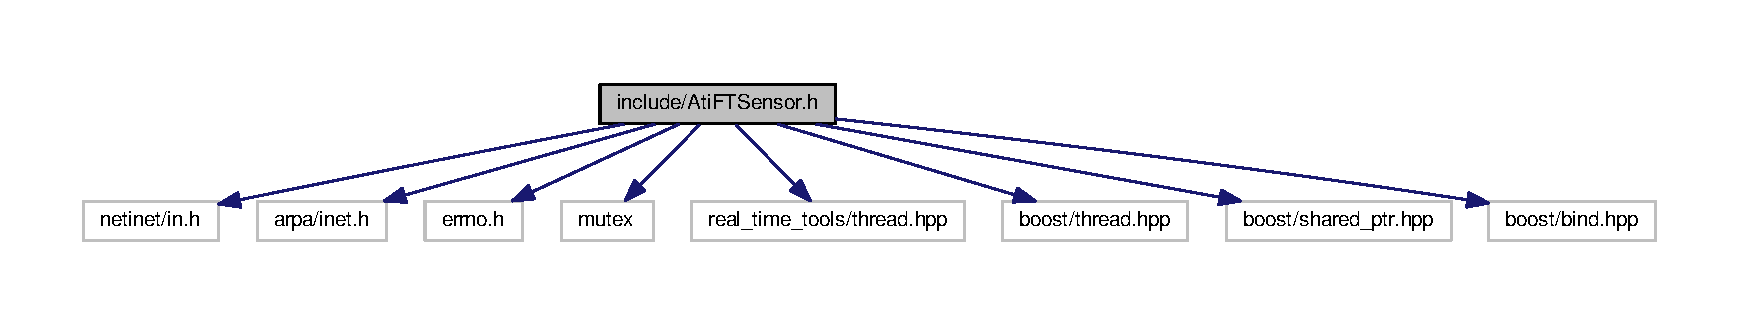
\includegraphics[width=350pt]{AtiFTSensor_8h__incl}
\end{center}
\end{figure}
\subsection*{Classes}
\begin{DoxyCompactItemize}
\item 
class \hyperlink{classati__ft__sensor_1_1AtiFTSensor}{ati\+\_\+ft\+\_\+sensor\+::\+Ati\+F\+T\+Sensor}
\item 
struct \hyperlink{structati__ft__sensor_1_1AtiFTSensor_1_1received__msg}{ati\+\_\+ft\+\_\+sensor\+::\+Ati\+F\+T\+Sensor\+::received\+\_\+msg}
\item 
struct \hyperlink{structati__ft__sensor_1_1AtiFTSensor_1_1send__msg}{ati\+\_\+ft\+\_\+sensor\+::\+Ati\+F\+T\+Sensor\+::send\+\_\+msg}
\end{DoxyCompactItemize}


\subsection{Detailed Description}
\begin{DoxyAuthor}{Author}
Ludovic Righetti 
\end{DoxyAuthor}
\begin{DoxyRefDesc}{License}
\item[\hyperlink{license__license000001}{License}]License B\+S\+D-\/3-\/\+Clause \end{DoxyRefDesc}
\begin{DoxyCopyright}{Copyright}
Copyright (c) 2019, New York University and Max Planck Gesellschaft. 
\end{DoxyCopyright}
\begin{DoxyDate}{Date}
2013-\/10-\/22 
\end{DoxyDate}

%--- End generated contents ---

% Index
\backmatter
\newpage
\phantomsection
\clearemptydoublepage
\addcontentsline{toc}{chapter}{Index}
\printindex

\end{document}
